% Title: Report LaTex File: Hardware Development
% Auther: DC Eksteen
% Student Number: 22623906
% Contact: 22623906@sun.ac.za
% Date: 2022/09/14
% Version: 2.0

\chapter{Hardware Development}

\section{Expected Force Calculations}

\newpage
\section{Eddy Current Brake Design}

The Eddy Currents in the Aluminium disc will be:
\[
	\acs{I}_e = \frac{\acs{condDisk} \acs{B} \acs{v}}{2}
\]
The eddy currents within the disc is then:
\[
	di = \frac{\acs{I}_e}{2 \pi} d\acs{theta}
\]
Using Ampere's Law, the force on an element at length l is then:
\[
	d\acs{F} = \acs{B} \, di \, dl
\]
\[
	d\acs{T} = l \, d\acs{F}
\]
Thus, combining all these, we get:
\[
	d\acs{T} = \frac{\acs{B} \, \acs{I}_e}{2 \pi} \, l \, d\acs{theta} \, dl
\]
By integrating, we get:
\[
	\int_{0}^{R} \int_{0}^{2 \pi} \frac{\acs{B} \, \acs{I}_e}{2 \pi} \, l \, d\acs{theta} \, dl
\]
\[
	\acs{T} = \frac{\acs{condDisk}\acs{B}^2\acs{omega}_n R^2}{6}
\]

\begin{figure}[H]
	\begin{center}
		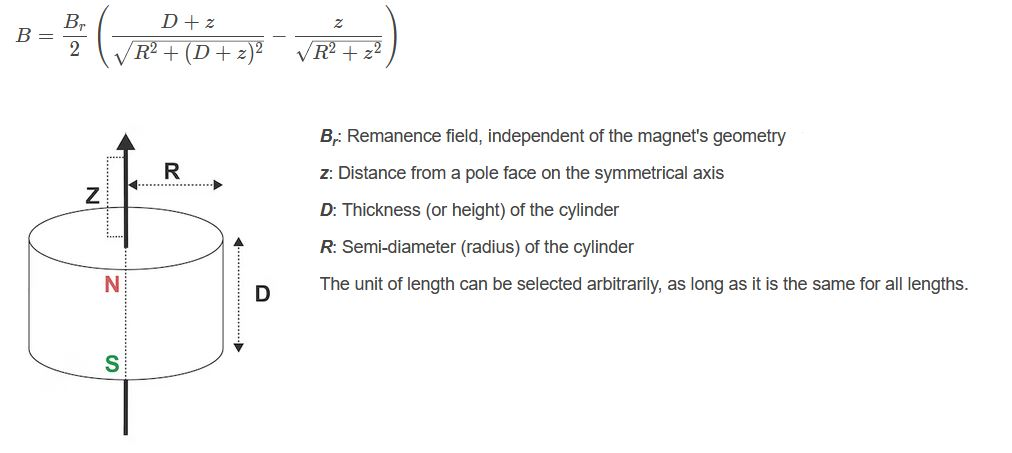
\includegraphics[width=0.8\textwidth]{Bfieldcalc.jpg}
		\caption{Magnetic Flux Density of Disc Magnet (adapted from: \citep{Supermagnete:2010})}
		\label{fig:B0}
	\end{center}
\end{figure}

\begin{figure}[H]
	\begin{center}
		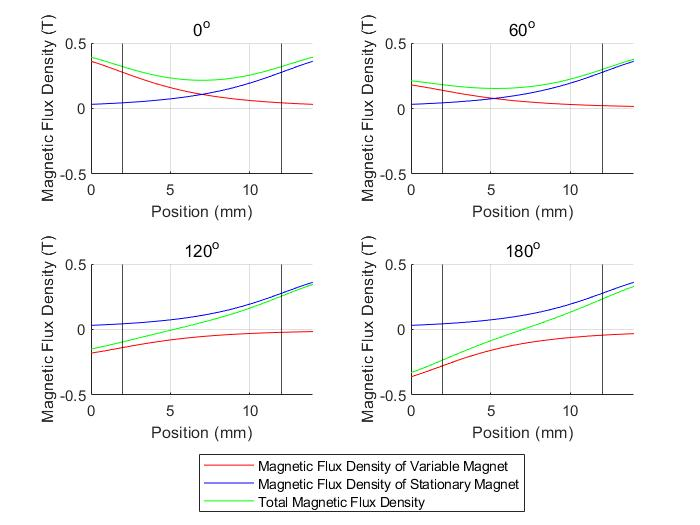
\includegraphics[width=\textwidth]{FluxDensityPhases.jpg}
		\caption{Magnetic Flux Density as Phase Changes}
		\label{fig:fluxD0}
	\end{center}
\end{figure}


$\frac{0.65\,{\left(0.001\,x-0.014\right)}}{\sqrt{{{\left(0.001\,x-0.014\right)}}^2 +0.000056249999999999998460432915070584}}-\frac{0.65\,{\left(0.001\,x-0.019\right)}}{\sqrt{{{\left(0.001\,x-0.019\right)}}^2 +0.000056249999999999998460432915070584}}$